\section{Overview}
\label{sec:orbweaver-intro}

% \begin{wrapfigure}{r}{0.5\textwidth}
%         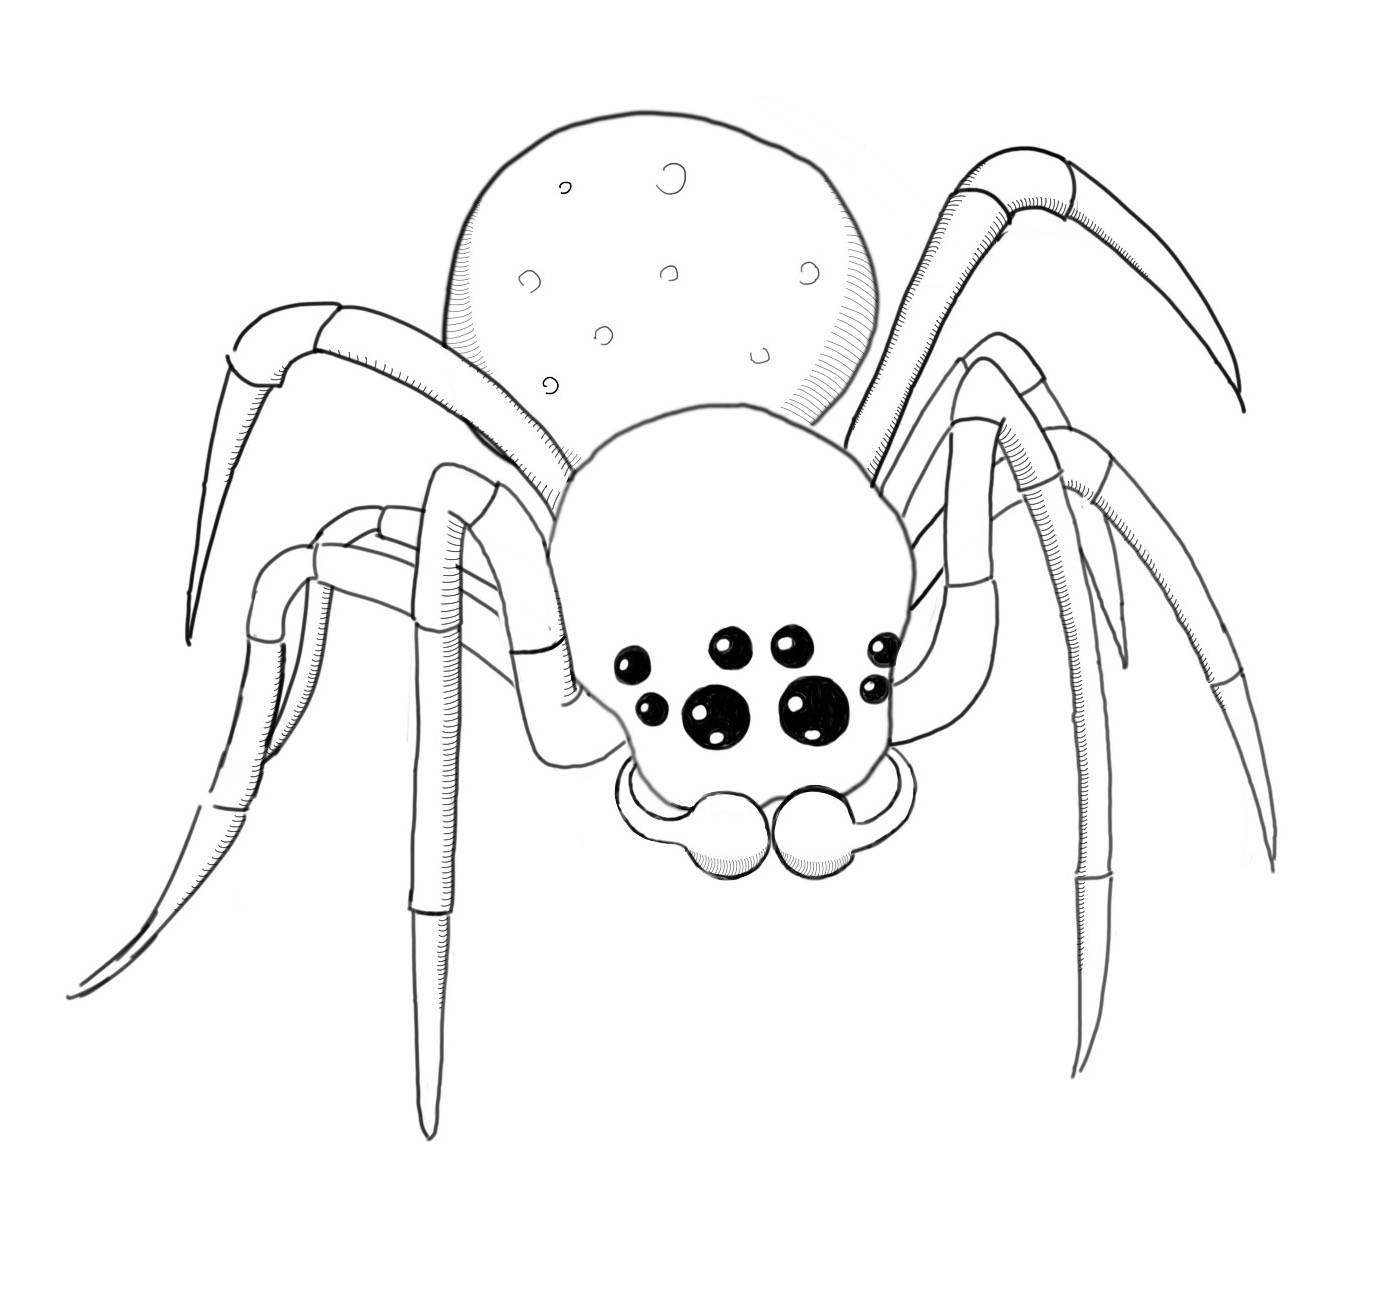
\includegraphics[width=0.48\textwidth]{spidey}
%         \captionsetup{labelformat=empty}
%         \caption{Lattice Orbweaver (Araneus thaddeus) by Jackie P (CC BY 4.0)}
% \end{wrapfigure}
Over the last decade there has been tremendous progress 
in the development succinct non-interactive argument of knowledge protocols,
called SNARKs~\cite{ITCS:BCCT12}.
For a public arithmetic circuit $C$ and a public input $\mathsf{x}$, 
these SNARKs enable a prover to convince a verifier
that the prover knows a witness $\mathsf{w}$ such that $C(\mathsf{x},\mathsf{w}) = 1$, where:
\begin{itemize}[nosep]
\item the proof is short, its length is at most 
$\text{poly}(\log \abs{C},\ \abs{\mathsf{x}},\ \lambda)$;
\item the proof can be verified in time 
$\text{poly}(\log \abs{C},\ \abs{\mathsf{x}},\ \lambda)$; and
\item generating the proofs takes quasilinear time in $\abs{C}$.
\end{itemize}
Here $\abs{C}$ is the number of gates in $C$,
and $\lambda$ is a security parameter.
The logarithmic dependence on $\abs{C}$ makes these proofs
remarkably short and fast to verify. 
Since the verifier needs to at least read $C$, 
there is also a 
one-time pre-processing phase applied to the circuit $C$.
Once pre-processed, the prover can provide proofs for many~$x$. 

Beyond knowledge of a witness, 
many of these proof systems can be efficiently extended to also
provide zero-knowledge.  
This progress generated considerable real-world interest,
and there are now implemented SNARKs and zkSNARKs capable of handling
statements involving many millions of arithmetic 
gates that are now deployed in real-world applications
(e.g.,~\cite{SP:BCGGMT14}).
%Here we focus on a SNARK construction, and leave the (somewhat standard) extension to a zkSNARK to the full version. \ben{TODO or remove} 

There are multiple techniques for constructing a pre-processing SNARK.
%(see~\cite{???} for an overview).
Some require a trusted setup~\cite{AC:Groth10a,TCC:Lipmaa12,STOC:BCCT13,EC:GGPR13,SP:PHGR13,TCC:BCIOP13,EC:Groth16,C:GroMal17,CCS:MBKM19,EPRINT:GabWilCio19,EC:CHMMVW20} where a trusted party must honestly generate public parameters. This setup is called \emph{universal} if it is not specific to the circuit $C$, i.e., it can be done once to generate parameters that can be used to preprocess any circuit $C$ in a publicly verifiable way. 
%If the trusted party is dishonest, the system becomes unsound.  
Other systems, called transparent SNARKs, require no trusted setup~\cite{C:BBHR19,EPRINT:BunFisSze19,EPRINT:ChiOjhSpo19,EPRINT:BowGriHop19}. 
%These systems rely on a verifiable linear-time pre-processing step 
%to process the statement, after which verification is logarithmic
%in the size of the statement.
%In this work we focus on transparent SNARKs since they are the most desirable in practice. 
\footnotetext{Named for the lattice orbweaver spider (araneus thaddeus).}
Many of the existing SNARKs %~\cite{EPRINT:BunFisSze19}
make use of a commitment scheme called a {\em polynomial commitment}~\cite{AC:KatZavGol10}, or PC.  A polynomial commitment enables a prover to commit to a polynomial $f \in \mathbb{F}[x]$ of degree $w$ using a short commitment.  Later, given two public values $\alpha, \beta \in \mathbb{F}$, the prover can convince a verifier that the committed polynomial $f$ satisfies $\beta = f(\alpha)$ and that $f$ has degree at most~$w$.  Ideally, the prover can verifiably open the polynomial at any point $\alpha \in \field$ using a short proof that can be efficiently checked. In fact, it has been shown that given polynomial commitment scheme with proof size $S(w)$ and verification time $T(w)$ it is possible to construct SNARKs with the same complexity characteristics in $w$ (the length of the witness), and additional complexity dependent only on a security parameter $\lambda$~\cite{EC:BunFisSze20, EC:CHMMVW20}. This compilation is in the random oracle model and relies on the Fiat-Shamir transform. %This paradigm led to several recent SNARK systems with improved characteristics, including very efficient pre-processing SNARKs with a  universal trusted setup~\cite{CCS:MBKM19,EC:CHMMVW20,EPRINT:GabWilCio19} or no trusted setup~\cite{EC:BunFisSze20}.


Polynomial commitment schemes are a special case of \emph{linear functional vector commitments}, where the prover has a commitment $C = \textsf{com}(\mathbf{x})$ to a vector $\mathbf{x} \in \mathbb{Z}_p^w$ and is able to open any linear form $f(\mathbf{x}) = \sum_{i = 1}^w \mathbf{x}_i f_i \bmod p$. Polynomial commitments, and the more general linear vector commitments, have been built from bilinear pairings~\cite{AC:KatZavGol10}, groups of unknown order~\cite{EPRINT:BunFisSze19}, proofs of proximity for Reed-Solomon codes~\cite{ICALP:BBHR18}, and to some degree from lattice-based assumptions~\cite{C:ACLMT22}. However, thus far all lattice-based constructions have had significant drawbacks, and none have achieved asymptotically (in the polynomial's degree) a quasilinear prover time with logarithmic proof size and logarithmic verification time. There are lattice-based generalizations of Bulletproofs~\cite{EC:BCCGP16,SP:BBBPWM18} based on the Ring-SIS assumption, which achieve quasilinear prover time and a polylogarithmic proof size, but have linear verification time~\cite{C:BLNS20,C:AttCraKoh21,C:AlbLai21}. Recently, \cite{C:ACLMT22} constructed general degree-$d$ polynomial map vector commitments (which include linear functions $d = 1 $ as a special case), which achieve logarithmic proof size and verification time, but have a CRS size and prover runtime that is at least $\Omega(w^{2d})$, and thus quadratic in the vector length for linear functions. This construction requires a trusted setup using lattice trapdoor sampling~\cite{EC:MicPei12}, and is based on $k\text{-}R\text{-}\mathsf{ISIS}$, a new family of lattice-based knowledge assumptions related to Ring-SIS. Another recent work, LaBRADOR~\cite{BS22}, uses recursion to achieve very compact proof sizes, but has verification time linear in $w$.

Polynomial commitment schemes based on codes and lattice assumptions are of particular importance due to their plausible post-quantum security. Constructions based on Reed-Solomon codes have quasilinear prover time and both polylogarithmic proof size and verifier time. So far they outperform any lattice-based construction not only asympotically, but also concretely by orders of magnitude in overall size and verification time, even when compared with recent lattice-based constructions that sacrifice prover performance for shorter proofs. Moreover, in the random oracle model, code-based constructions use weaker  assumptions than lattice-based constructions. Nonetheless, we are optimistic that the additional structure lattices provide vs. generic (i.e., hash and code-based) constructions can be exploited such that lattice SNARKs eventually surpass these results. As a point of reference, hash-based signatures were originally more efficient, but after over a decade of development lattice-based signatures are an order of magnitude smaller and two faster.

A primary motivation of recent lattice-based constructions~\cite{C:ACLMT22,WW22} of vector commitments supporting higher degree polynomial map openings is that, unlike linear function commitments, they can be used to build SNARKs more directly (e.g., by opening an R1CS form) without invoking the Fiat-Shamir transform. Unfortunately, current approaches to supporting higher degree polynomial maps seem to fundamentally require a quadratic prover time. Given the additional structure of lattices compared with code-based proof systems that rely only on hash functions, one might expect that it would be possible to obtain smaller proof sizes and faster verification times. The recent work LaBRADOR~\cite{BS22} was the first lattice-based system to achieve proof sizes smaller (both concretely and asymptotically) than code-based systems, but this has not yet been done for combined proof size and verification time. The results of this paper make progress in this direction. 